{\color{gray}\hrule}
\begin{center}
\section{Background And Description}
\bigskip
\end{center}
{\color{gray}\hrule}
\begin{multicols}{2}

You Only Look Once (YOLO) is a real-time object detection neural network that has multiple areas of applications in computer vision tasks. The framework was introduced in 2015 by Joseph Redmond, a PhD candidate who successfully demonstrated his expertise in the field of computer science and mathematics while attending Middlebury College, where he simultaneously served as the Computer Science tutor and worked at National Institute of Standards and Technology. The YOLO machine learning algorithm made a major leap forward in the computer vision field, bringing a new method of localizing and categorizing an object in a single shot, which resulted in a higher operating speed than its predecessors. 

Previously, the major models of real-time object detection such as R-CNN, Fast R-CNN and Faster R-CNN relied on two-stage method and regionally proposal-based categorization which could only achieve up to 5 frames per second (FPS) operation, lacking the processing capabilities to analyze the real-time images captured at 30-fps or more. Unlike the R-CNN model, YOLO processed the entire image in one forward pass, avoiding multiple stages of breaking down the detection process into multiple steps, that included finding the regions and then classifying each field.

\subsection{YOLOv1}
The architecture of the YOLOv1 model is called - “Darknet” framework, and it is mainly inspired by the GoogNet model, whose structure consists of 24 layers following 2 fully connected layers: See \ref{fig:Darknet Framework}. The whole concept of object detection is framed as a regression problem, rather than a region proposal network with classification stage. This approach enabled YOLOv1 to capture the bounding boxes coordinates (location) and class probability (object classification) in a single attempt, treating the object detection as a unified task. The method is based on a mathematical technique called mean square error, which measures the distance between the guesses and the truth, making the process fast and therefore suitable for use in real time. In the model, the input image is divided into a 7x7 grid cell, where each cell predicts two factors: the first is the 2 bounding boxes for each cell, and the second is a confidence score that provides the level of confidence in the existence of an object inside the cell and the accuracy of the object in matching the predicted feature. To calculate the confidence score, a technique called - Intersection over Union (IoU) is used to filter the predictions and the formula for each grid cell is provided as follows Pr(object) * IOU (truth, pred). This is the overlapping area of two intersecting regions - ground truth and predicted boxes divided by the area of their union. If the high confidence score was captured after filter prediction, then these fields are checked against ground truth to decide if they are True Positive (TP), or False Positive (FP). However, despite such outperforming results of YOLOv1 neural network, some characteristics of the model struggle to accurately identify tightly grouped objects within an image as well as small, distant objects. The solution is discussed further in this research
\end{multicols}

\begin{figure}[ht]
    \centering
    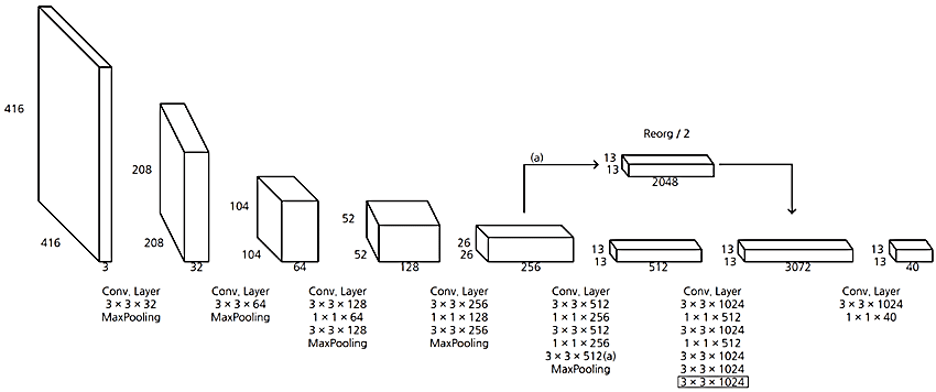
\includegraphics[width=0.9\linewidth]{datas/Darknet Framework.png}
    \caption{Darknet Framework, combination of 24 layers with 2 fully connected layers.}
    \label{fig:Darknet Framework}
\end{figure}

\begin{multicols}{2}
\subsection{YOLOv2}
Although YOLOv1 introduced object detection as a single regression problem, the limitations of this novel concept influenced the release of the new version - YOLOv2, also known as YOLO9000. The next stage of evolution was focused on improving existing weaknesses of the model, as well as improving accuracy without sacrificing the speed. Such upgrades led to the implementation of multiple features that are built on the foundation of YOLOv1. The new design of Darknet-19 architecture consists of 19 convolutional layers following 5 max-pooling layers. Reducing parameters by 60\%, while maintaining accuracy, which only required 5.58 billion operations to process an image. The bounding box prediction achieved better prediction results after incorporating anchor box prediction, a predefined set of boxes with different aspect ratios and scale. Instead of predicting the coordinates of each cell, the RPN predicts the offset of across the grid. Additionally, each convolutional layer adopted batch normalization technique, resulting in over 2\% improvement in mean Average Precision (mAP). YOLOv2 also makes effective use of the multi-scale method — a process of training the model on images at different scales to average the prediction, improving the detection of small objects.



\subsection{YOLOv3}
The third version of YOLO model proposed a new Darknet-59 backbone architecture which is made of 53 convolutional layers and incorporates residual blocks that vary from 3x3 to 1x1 layers (13x13, 26x26. 52x52). 

By integrating the Pyramid architecture, which closely resembles the Feature Pyramid Network (FPN), it effectively manages a feature map at three different resolutions, each of which is analyzed to produce a separate prediction grid. Thus, the model applies detection mechanisms more efficiently to objects of different sizes. Overall, YOLOv3 achieved better results compared to its precursor, which is deeper and more robust with improved data-loading performance.

\subsection{YOLOv4}
The release of YOLOv4 brought significant improvements to the architecture, shifting to a new CNN architecture named Cross Stage Partial Network (CSPNet), with the design of 54 layers, splitting the structure into three separate components: backbone, neck, and head, and each responsible for its own distinct feature, see \ref{fig:CSPNet}. The backbone employs convolutional neural networks to learn features throughout all layers. The neck part serves as a basis which is formed based on extracted features gathered across different layers. Finally, the head processes bounding box prediction, and works on class probabilities. One of the primary updates included in the fourth generation of the YOLO model revolves around the optimization, involving Mosaic Data Augmentation which combines 4 images rolled into one, increasing the number of contexts scenarios where object detection would work. Self-Adversarial Training (SAT) is designed to improve robustness and generalization, which makes the model think there is no object, with the double staged data augmentation approach. Cross-mini Batch Normalization (CmBN) optimizes the single GPU utilization during the training. Modified Spatial Attention Model (MSAM) helps the model focus on crucial features with no cost on the performance. 
\end{multicols}

\begin{figure}[ht]
    \centering
    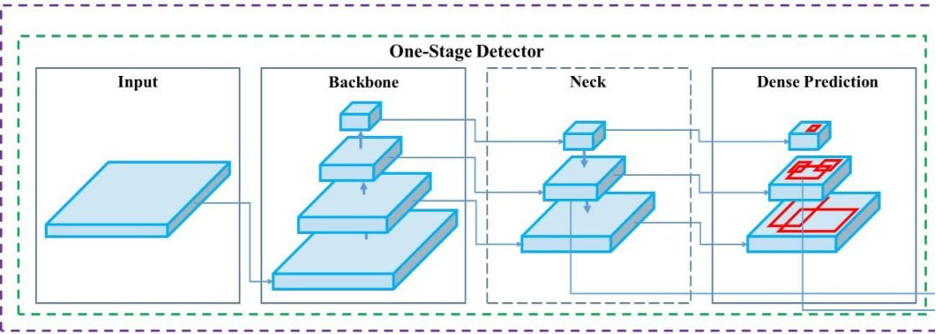
\includegraphics[width=1\linewidth]{datas/Cross Stage Partial Network (CSPNet).png}
    \caption{Cross Stage Partial Network (CSPNet), a 54 layered architecture with 3 separate components: Backbone, Neck and Head.}
    \label{fig:CSPNet}
\end{figure}
 
\begin{multicols}{2}
\subsection{YOLOv5}
Aiming for the better performance-wise benchmarks, an incremental advancement YOLOv5 was designed based on the previous version. Mainly, the developers focused on user-friendly aspects, simplifying model implementation and making the documentation more accessible by supporting multiple languages, and finally, the entire model was built on the PyTorch framework, making the technology more straightforward in application. 

Furthermore, transferring to a more complex architecture similar to the EfficientNet network framework called EfficientDet. The results of this change presents higher accuracy results, better generalization, and wider range of object categorization. Additionally, the new version presents a new pooling technique - Spatial Pyramid Pooling (SPP), which reduces the spatial scaling across the grid, which effectively detects objects of a smaller size. 


\subsection{YOLOv6}
The release of YOLOv6 has influenced application in the industrial sector, offering nicely tuned performance between speed and accuracy rate. Along with the architecture enhancement, the model incorporates Bi-directional Concatenation (BiC), Anchor-aided training (AAT) scheme, and the improved neck component. A newer version of architecture, EfficientNet-L2 required a smaller number of parameters, and received large processing power. The AAT strategy utilized an anchor-based method, accompanied by the anchor-free technique, which proposed a method that does not rely on a predefined set of anchor boxes with different resolutions, but only predicts the locations of center points and corner key points derived from the image features. Thus, expanding the capabilities of the detection mechanism. The BiC module is a part of the neck component that results in performance gains, by directly influencing the localization signals in the neck component. This iteration of YOLO has adopted several strategies to better optimize the computation of the model. For instance, during the training phase of the neural network, it assigns the labels to the predefined anchor boxes. Usually, this happens with the help of multiple strategies and of varying complexity. Including IoU method, ground-truth based technique, or SimOTA label assignment.

\subsection{YOLOv7}
Designers of YOLOv7 focused on refining the capabilities of previous versions, along with alternative technologies, demonstrating satisfying benchmarks. One of the major improvements is the increased FPS rates of the real-time image, achieving up to 155 frame per second processing. Making significant progress in the field of real-time detection, especially in time-sensitive scenarios such as autopiloting and surveillance. This generation of the model requires 50\% less computing load and decreases in the number of parameters as well by 40\%, achieving higher accuracy without an inference cost raise. In general, this version is considered as one of the fastest among leading alternatives in the field. By incorporating dynamic label assignments, extended and compound scaling and re-parameterization, it demonstrates satisfying benchmarks.

\subsection{YOLOv8}
YOLOv8 is one of the major and stable versions of the model, it involves advanced backbone and neck architecture. Offering a variety of pre-trained models where each designed for specific task, including object detection, instance segmentation, oriented object detection pose/keypoints detection and classification. In this generation, YOLOv8 avoided using an anchor-based approach, but instead took advantage of the anchor free method, relying on predicting the object centers. In terms of performance, it achieved cutting-edge results of 37.3 on the mAP score tested on COCO dataset with speed of 0.99ms using A100 TensorRT GPU. As of today, YOLOv8 remains widely used among many computer vision algorithms.

\subsection{YOLOv9}
The release of YOLOv9 marked a pivotal step in the deep neural network area, introducing highly effective solutions to the long-lasting challenges, by implementing a new innovative architecture called Generalized Efficient Layer Aggregation Network, or GELAN for short, and feature named - Programmable Gradient Information (PGI), incorporating these two essential enhancements, the model is able to address the issue data loss, improving the model retention and training capabilities. In the deep neural network, it is often the case when the data is passed deeper through the layers, but the more it goes on, the chances of information being lost increases. The application of PGI helps in avoiding by ensuring the integrity of the crucial data throughout all layers of the network. Compared to the previous generation, YOLOv9 demands even less computing and number of parameters, which are 25\% and 15\%, respectively. Generally, this generation of YOLO brings effective architecture design, improved accuracy and adaptability.

\subsection{YOLOv10}
YOLOv10 addressed the design flows of past YOLO iterations by becoming independent of post-processing tools such as non-maximum suppression (NMS) and refining the architectural structure to gain additional components, including a one-to-many head and a one-to-one head, in addition to the backbone and neck components that received upgrades as well. Better gradient flow, improved version of CSPNet, and decreased workload. The YOLOv10 takes advantage of the new key feature called dual assignment, employing both one-to-one and one-to-many techniques in the detection pipeline, where One-to-Many in the training phase, works with multiple predictions based on a single object and improves the learning curve. While One-to-One components reduce the latency by creating the prediction with the highest confidence score possible during the inference, resulting in efficiency gain. Together, these two modules make appropriate conditions to eliminate NMS technique.

\subsection{YOLOv11}
Currently, YOLOv11 remains one of the stable and commonly used versions in the family of YOLO models, being widely used in the industry and the community. Built over the last iterations of YOLOs, the 11th generation has achieved exceptional accuracy, speed and efficiency characteristics. Among the involved significant changes were the Enhanced Feature Extraction algorithm, redesign of architectural scheme, newer versions of feature pipelines, environment adaptability, and integrated wide range of varying tasks in the computer vision sector. The unique aspect of new architectural design is the implementation of components such as C3k2 Block and C2PSA Block minimizing the redundant computation and the number of parameters. C3k2 Block replaces the block of C2f block, dividing the structure of convolution into 2 convolutions but of a smaller scale. This approach showcased efficient wise boost compared to the CSP bottleneck. The purpose of C2PSA Block is to implement an attention mechanism that focuses around the most relevant regions across the image. Extracting the features on the smaller objects and within low-visible areas.
The model achieved cutting-edge performance metrics among the available models. 

In comparison, the 8th generation of YOLO, which is considered one of the stable versions among YOLO series, is outperformed by YOLOv11 in terms of feature extraction and processing metrics, being higher on mean Average Precision (mAP) using 22\% less parameters during the COCO dataset testing. Although both support versatile types of computer vision operations, but general accessibility of YOLOv11 makes a determining factor in choosing for this research, being environment-friendly system and requiring less parameters for testing

\subsection{YOLOv12}
At the time of writing, the YOLOv12 is the latest version available on February 18th, 2025. The major difference to the past generations of YOLOs, is the reconceptualized architecture of CNN, built over the years since YOLOv1. The novel approach in this architecture is an area attention mechanism, which splits the feature map into S equal sized areas. The idea is to avoid excessive complexity, reducing redundant workload. To address optimization challenges, Residual Efficient Layer Aggregation Networks (R-ELAN) was introduced as a novel method of feature aggregation, and block-level residual connections. As every model iteration, it improves over its predecessor in efficient utilization, accuracy, and performance load.

\end{multicols}